\includepdf[pages=-]{"Temas/Tema 1/Hoja 1"}

\begin{enumerate}[label=\color{red}\textbf{\arabic*)}, leftmargin=*]
	\item \lb{Exprese cada uno de los siguientes números complejos en su parte real e imaginaria $(a+jb)$: \[ \dfrac{1}{2}e^{j\pi},\frac{1}{2}e^{-j\pi},e^{j\frac{\pi}{2}},e^{j-\frac{\pi}{2}},e^{j\frac{5\pi}{2}},\sqrt{2}e^{j\frac{\pi}{4}},\sqrt{2}e^{j\frac{9\pi}{4}},\sqrt{2}e^{-j\frac{9\pi}{4}},\sqrt{2}e^{-j\frac{\pi}{4}} \]}
	\item \lb{Exprese cada uno de los siguientes números complejos en su módulo y fase $\left(|z|e^{j\varphi(z)}\text{ con }\varphi(z)\in[-\pi,\pi]\right)$: \[ 5,-2,-3j,-j\dfrac{\sqrt{3}}{2},1+j,(1-j)^2,j(1-j),\dfrac{1+j}{1-j},\dfrac{\sqrt{2}+j\sqrt{2}}{1+j\sqrt{3}} \]}
	\item \lb{Calcule los valores de potencia media y de energía de las siguientes señales}
	\begin{enumerate}[label=\color{red}\alph*)]
		\item $\db{x(t)=e^{-2t}u(t)}$

		\begin{tikzpicture}[baseline=(current bounding box.center)]
			\draw (-2,0) -- (3,0);
			\draw (0,-1) -- (0,1.5);
			\draw[lightblue, line width=1.5pt] (-2, 0) -- (0,0) -- (0,1);
			\draw[lightblue, line width=1.5, domain=0:3] plot (\x, {e^(-\x)});
		\end{tikzpicture}\qquad\begin{minipage}{0.45\textwidth}
			$\displaystyle E_T=\infi|x(t)|^2\dt=\int_{0}^{+\infty}|e^{-2t}|^2\dt=\int_{0}^{+\infty}e^{-4t}\dt=\left[-\dfrac{1}{4}e^{-4t}\right]_{0}^{+\infty}=-\dfrac{1}{4}\left[0-1\right]=\dfrac{1}{4}J$
		\end{minipage}

		$P_m=\lim_{T\to+\infty}\dfrac{1}{2T}\lbb{\int_{-T}^{T}|x(t)|^2\dt}{E_T}=\lim_{T\to+\infty}\dfrac{1}{2T}\cdot E_T=\dfrac{\frac{1}{4}}{+\infty}=0$
		\item $\db{x(t)=e^{j\left(2t+\frac{\pi}{4}\right)t}}$

		$E_T=\infi\left|e^{j\left(2t+\frac{\pi}{4}\right)t}\right|^2\dt=\infi1^2\dt=\left[t\right]_{-\infty}^{+\infty}=\infty+\infty=\infty$

		$P_m=\dfrac{1}{T}\int_{-\frac{T}{2}}^{\frac{T}{2}}\left| e^{j\left( 2t+\frac{\pi}{4} \right)t}\right|^{2}\:\mathrm{d}t=\int_{-\frac{T}{2}}^{\frac{T}{2}}\:\mathrm{d}t=\left[ \dfrac{t}{T} \right]_{-\frac{\pi}{2}}^{\frac{\pi}{2}}=\dfrac{\dfrac{\pi}{2}+\dfrac{\pi}{2}}{T}=1W$
		\item $\db{x(t)=\cos(t)}$

		$E_{T}=\int_{-\infty}^{\infty}\left| \cos(t) \right|^2\:\mathrm{d}t=\int_{-\infty}^{\infty} \cos^{2}(t)=\left\{ \cos^{2}(\alpha)=\dfrac{1}{2}\left[ 1+\cos(2\alpha)\right] \right\}=\int_{-\infty}^{\infty} \dfrac{1}{2}(1+\cos(2t))=\left[\dfrac{1}{2}t+\dfrac{1}{4}\sin(2t)\right]=\infty$

		$P_{m}=\dfrac{1}{T}\int_{-\frac{T}{2}}^{\frac{T}{2}}\cos^{2}(t)\:\mathrm{d}t=\dfrac{1}{2t}\left[ t+\dfrac{\sin(2t)}{2} \right]_{-\frac{\pi}{2}}^{\frac{\pi}{2}}=\dfrac{1}{2t}\left[ \dfrac{\pi}{2}+\dfrac{\pi}{2}+\dfrac{\sin(T)-\sin(-T)}{2} \right]=\dfrac{1}{2T}\left[ T+\tozero{\sin(T)}~~~ \right]=\dfrac{1}{2}W$

		$T=\dfrac{2\pi}{\omega_{0}}=\dfrac{2\pi}{1}=2\pi$
		\item $\db{x[n]=\left(\dfrac{1}{2}\right)^nu[n]}$

		\begin{center}
			\begin{tikzpicture}[scale=1.5]

				\draw[->] (-2.5,0) -- (5,0) node[right] {$n$};
				\draw[->] (0,-1) -- (0,2) node[above] {$x[n]$};

				\foreach \x in {1,...,4}
				\draw (\x,0.1) -- (\x,-0.1) node[below] {\x};

				\foreach \x in {0,...,4}
				\fill[lightblue] (\x,{pow(0.5,\x)}) circle (1.5pt);

				\draw[domain=0:5, samples=150, lightblue] plot (\x, {pow(0.5,\x)});
				\draw[lightblue] (-2,0) -- (0,0) -- (0,1);

				\foreach \x in {-2,-1}
				\fill[lightblue] (\x,0) circle (1.5pt);
			\end{tikzpicture}
		\end{center}
		$E_{T}=\sum_{n=-\infty}^{\infty}|x[n]|^2=\sum_{n=0}^{\infty}\left| \left( \dfrac{1}{2} \right)^{n} \right|^2=\sum_{n=0}^{\infty}\left( \dfrac{1}{2} \right)^{2n}=\dfrac{1-0\cdot\frac{1}{4}}{1-\frac{1}{4}}=\dfrac{4}{3}J$
		\item $\db{x[n]=e^{j\left(\frac{\pi}{2n}+\frac{\pi}{8}\right)}}$

		$E_T=\sum_{n=-\infty}^\infty \left|e^{j\left( \pi/2n+\pi/8 \right)} \right|^2=\sum_{n=-\infty}^\infty1=\infty$

		$P_m=\dfrac{1}{N}\sum_{n=0}^{N-1}\left| x[n] \right|^2=\dfrac{1}{4}\sum_{n=0}^31=\dfrac{4}{4}=1 N$

		$\omega_0=\dfrac{\pi}{2}\longrightarrow N=\dfrac{2\pi}{\omega_0}K=4K=\left\{ K=1 \right\}=4$
		\item $\db{x[n]=\cos\left(\dfrac{\pi}{4}n\right)}$

		$E_T=\sum_{n=-\infty}^\infty \cos^2\left( \dfrac{\pi}{4}n \right)=\infty$\\
		$P_m=\dfrac{1}{N}\sum_{n=0}^{N-1}\cos^2\left( \dfrac{\pi}{4}n \right)=\dfrac{1}{8}\sum_{n=0}^7\dfrac{1}{2}\left[ 1+\cos \left( \dfrac{\pi}{2}n \right) \right]=\left\{ \begin{array}{ll}n=0\to 1 & n=4\to 1\\ n=1\to 0&n=5\to 0\\ n=2\to -1 & n=6\to -1\\ n=3\to 0 & n=7\to 0\end{array} \right\}=\dfrac{8}{16}=\dfrac{1}{2}W$\\
		$\omega_0=\dfrac{\pi}{4}\longrightarrow N=\dfrac{2\pi}{\omega_{0}}K=8K=\left\{ K=1 \right\}=8$
	\end{enumerate}
	\item \lb{Considere una señal $x[n]$ en la que $x[n]=0$ para $n<-2$ y $n>4$. Para cada una de las señales siguientes determine los valores de $n$ en los que se garantiza que la señal es cero.}

	\begin{tikzpicture}[scale=0.75]
		\draw[->] (-10.5,0) -- (10.5,0) node[right] {$n$};
		\draw[->] (0,-1) -- (0,5) node[above] {$x[n]$};
		\foreach \y in {-1,0,...,5} {
				\draw (0.1,\y) -- (-0.1,\y);
			}
		\foreach \x in {-10,...,-3}{
				\fill[lightblue] (\x,0) circle (2pt);
			}
		\foreach \x in {5,...,10}{
				\fill[lightblue] (\x,0) circle (2pt);
			}
		\foreach \x in {-10,...,10}{\node[below] at (\x,0) {$\x$};}
		\fill[lightblue] (-2,1) circle (2pt);
		\fill[lightblue] (-1,2) circle (2pt);
		\fill[lightblue] (0,4) circle (2pt);
		\fill[lightblue] (1,5) circle (2pt);
		\fill[lightblue] (2,5) circle (2pt);
		\fill[lightblue] (3,3.5) circle (2pt);
		\fill[lightblue] (4,2) circle (2pt);
		\draw[lightblue, line width=1.2] (-2,0) -- (-2,1);
		\draw[lightblue, line width=1.2] (-1,0) -- (-1,2);
		\draw[lightblue, line width=1.2] (0,0) -- (0,4);
		\draw[lightblue, line width=1.2] (1,0) -- (1,5);
		\draw[lightblue, line width=1.2] (2,0) -- (2,5);
		\draw[lightblue, line width=1.2] (3,0) -- (3,3.5);
		\draw[lightblue, line width=1.2] (4,0) -- (4,2);
		\foreach \y in {0.2,0.4,0.6,0.8,1}{\node[left] at (0,{\y*5}) {$\y$};}
	\end{tikzpicture}
	\begin{enumerate}[label=\color{red}\alph*)]
		\item $\db{x[n-3]}$

		Vemos que esta señal se corresponde con un desplazamiento de 3 unidades a la derecha. Por tanto, $x[n-3]=0$ para $n<1$ y $n>7$.

		\begin{tikzpicture}[scale=0.75]
			\draw[->] (-10,0) -- (10,0) node[right] {$n$};
			\draw[->] (0,-1) -- (0,5) node[above] {$x[n-3]$};
			\foreach \x in {-10,-9,...,10} {
					\draw (\x,0.1) -- (\x,-0.1);
				}
			\foreach \y in {-1,0,...,5} {
					\draw (0.1,\y) -- (-0.1,\y);
				}

			\foreach \x in {-10,...,0}{
					\fill[lightblue] (\x,0) circle (2pt);
				}
			\foreach \x in {8,...,10}{
					\fill[lightblue] (\x,0) circle (2pt);
				}
			\foreach \x in {-10,...,10}{\node[below] at (\x,0) {$\x$};}
			\fill[lightblue] (1,1) circle (2pt);
			\fill[lightblue] (2,2) circle (2pt);
			\fill[lightblue] (3,4) circle (2pt);
			\fill[lightblue] (4,5) circle (2pt);
			\fill[lightblue] (5,5) circle (2pt);
			\fill[lightblue] (6,3.5) circle (2pt);
			\fill[lightblue] (7,2) circle (2pt);
			\draw[lightblue, line width=1.2] (1,0) -- (1,1);
			\draw[lightblue, line width=1.2] (2,0) -- (2,2);
			\draw[lightblue, line width=1.2] (3,0) -- (3,4);
			\draw[lightblue, line width=1.2] (4,0) -- (4,5);
			\draw[lightblue, line width=1.2] (5,0) -- (5,5);
			\draw[lightblue, line width=1.2] (6,0) -- (6,3.5);
			\draw[lightblue, line width=1.2] (7,0) -- (7,2);
			\foreach \y in {0.2,0.4,0.6,0.8,1}{\node[left] at (0,{\y*5}) {$\y$};}
		\end{tikzpicture}
		\item $\db{x[n+4]}$

		Veamos que esta señal se corresponde con un desplazamiento de 4 unidades a la izquierda. Por tanto, $x[n+4]=0$ para $n<-6$ y $n>0$

		\begin{tikzpicture}[scale=0.75]
			\draw[->] (-10.5,0) -- (10.5,0) node[right] {$n$};
			\draw[->] (0,-1) -- (0,5) node[above] {$x[n+4]$};
			\foreach \y in {-1,0,...,5} {
					\draw (0.1,\y) -- (-0.1,\y);
				}
			\foreach \x in {-10,...,-7}{
					\fill[lightblue] (\x,0) circle (2pt);
				}
			\foreach \x in {1,...,10}{
					\fill[lightblue] (\x,0) circle (2pt);
				}
			\foreach \x in {-10,...,10}{\node[below] at (\x,0) {$\x$};}
			\fill[lightblue] (-6,1) circle (2pt);
			\fill[lightblue] (-5,2) circle (2pt);
			\fill[lightblue] (-4,4) circle (2pt);
			\fill[lightblue] (-3,5) circle (2pt);
			\fill[lightblue] (-2,5) circle (2pt);
			\fill[lightblue] (-1,3.5) circle (2pt);
			\fill[lightblue] (0,2) circle (2pt);
			\draw[lightblue, line width=1.2] (-6,0) -- (-6,1);
			\draw[lightblue, line width=1.2] (-5,0) -- (-5,2);
			\draw[lightblue, line width=1.2] (-4,0) -- (-4,4);
			\draw[lightblue, line width=1.2] (-3,0) -- (-3,5);
			\draw[lightblue, line width=1.2] (-2,0) -- (-2,5);
			\draw[lightblue, line width=1.2] (-1,0) -- (-1,3.5);
			\draw[lightblue, line width=1.2] (0,0) -- (0,2);
			\foreach \y in {0.2,0.4,0.6,0.8,1}{\node[left] at (0,{\y*5}) {$\y$};}
		\end{tikzpicture}
		\item $\db{x[-n]}$

		Vemos que esta señal se corresponde con una reflexión o simetría de la señal con respecto al eje central. Por tanto, $x[-n]=0$ para $n<-4$ y $n>2$

		\begin{tikzpicture}[scale=0.75]
			\draw[->] (-10.5,0) -- (10.5,0) node[right] {$n$};
			\draw[->] (0,-1) -- (0,5) node[above] {$x[-n]$};
			\foreach \y in {-1,0,...,5} {
					\draw (0.1,\y) -- (-0.1,\y);
				}
			\foreach \x in {-10,...,-5}{
					\fill[lightblue] (\x,0) circle (2pt);
				}
			\foreach \x in {5,...,10}{
					\fill[lightblue] (\x,0) circle (2pt);
				}
			\foreach \x in {-10,...,10}{\node[below] at (\x,0) {$\x$};}
			\fill[lightblue] (-4,1) circle (2pt);
			\fill[lightblue] (-3,2) circle (2pt);
			\fill[lightblue] (-2,4) circle (2pt);
			\fill[lightblue] (-1,5) circle (2pt);
			\fill[lightblue] (0,5) circle (2pt);
			\fill[lightblue] (1,3.5) circle (2pt);
			\fill[lightblue] (2,2) circle (2pt);
			\draw[lightblue, line width=1.2] (-4,0) -- (-4,1);
			\draw[lightblue, line width=1.2] (-3,0) -- (-3,2);
			\draw[lightblue, line width=1.2] (-2,0) -- (-2,4);
			\draw[lightblue, line width=1.2] (-1,0) -- (-1,5);
			\draw[lightblue, line width=1.2] (0,0) -- (0,5);
			\draw[lightblue, line width=1.2] (1,0) -- (1,3.5);
			\draw[lightblue, line width=1.2] (2,0) -- (2,2);
			\foreach \y in {0.2,0.4,0.6,0.8,1}{\node[left] at (0,{\y*5}) {$\y$};}
		\end{tikzpicture}
		\item $\db{x[-n+2]}$

		Vemos que esta señal se corresponde con una reflexión o simetría de la señal respecto al eje central y un desplazamiento a la derecha de 2 unidades. Por tanto, $x[-n+2]=0$ para $n<-2$ y $n>4$

		\begin{tikzpicture}[scale=0.75]
			\draw[->] (-10.5,0) -- (10.5,0) node[right] {$n$};
			\draw[->] (0,-1) -- (0,5) node[above] {$x[-n+2]$};
			\foreach \y in {-1,0,...,5} {
					\draw (0.1,\y) -- (-0.1,\y);
				}
			\foreach \x in {-10,...,-3}{
					\fill[lightblue] (\x,0) circle (2pt);
				}
			\foreach \x in {5,...,10}{
					\fill[lightblue] (\x,0) circle (2pt);
				}
			\foreach \x in {-10,...,10}{\node[below] at (\x,0) {$\x$};}
			\fill[lightblue] (-2,1) circle (2pt);
			\fill[lightblue] (-1,2) circle (2pt);
			\fill[lightblue] (0,4) circle (2pt);
			\fill[lightblue] (1,5) circle (2pt);
			\fill[lightblue] (2,5) circle (2pt);
			\fill[lightblue] (3,3.5) circle (2pt);
			\fill[lightblue] (4,2) circle (2pt);
			\draw[lightblue, line width=1.2] (-2,0) -- (-2,1);
			\draw[lightblue, line width=1.2] (-1,0) -- (-1,2);
			\draw[lightblue, line width=1.2] (0,0) -- (0,4);
			\draw[lightblue, line width=1.2] (1,0) -- (1,5);
			\draw[lightblue, line width=1.2] (2,0) -- (2,5);
			\draw[lightblue, line width=1.2] (3,0) -- (3,3.5);
			\draw[lightblue, line width=1.2] (4,0) -- (4,2);
			\foreach \y in {0.2,0.4,0.6,0.8,1}{\node[left] at (0,{\y*5}) {$\y$};}
		\end{tikzpicture}
		\item $\db{x[-n-2]}$

		Vemos que esta señal se corresponde con una reflexión o simetría de la señal con respecto al eje central y un desplazamiento a la izquierda de 2 unidades. Por tanto, $x[-n-2]=0$ para $n<-6$ y $n>0$.

		\begin{tikzpicture}[scale=0.75]
			\draw[->] (-10.5,0) -- (10.5,0) node[right] {$n$};
			\draw[->] (0,-1) -- (0,5) node[above] {$x[-n-2]$};
			\foreach \y in {-1,0,...,5} {
					\draw (0.1,\y) -- (-0.1,\y);
				}
			\foreach \x in {-10,...,-7}{
					\fill[lightblue] (\x,0) circle (2pt);
				}
			\foreach \x in {1,...,10}{
					\fill[lightblue] (\x,0) circle (2pt);
				}
			\foreach \x in {-10,...,10}{\node[below] at (\x,0) {$\x$};}
			\fill[lightblue] (-6,1) circle (2pt);
			\fill[lightblue] (-5,2) circle (2pt);
			\fill[lightblue] (-4,4) circle (2pt);
			\fill[lightblue] (-3,5) circle (2pt);
			\fill[lightblue] (-2,5) circle (2pt);
			\fill[lightblue] (-1,3.5) circle (2pt);
			\fill[lightblue] (0,2) circle (2pt);
			\draw[lightblue, line width=1.2] (-6,0) -- (-6,1);
			\draw[lightblue, line width=1.2] (-5,0) -- (-5,2);
			\draw[lightblue, line width=1.2] (-4,0) -- (-4,4);
			\draw[lightblue, line width=1.2] (-3,0) -- (-3,5);
			\draw[lightblue, line width=1.2] (-2,0) -- (-2,5);
			\draw[lightblue, line width=1.2] (-1,0) -- (-1,3.5);
			\draw[lightblue, line width=1.2] (0,0) -- (0,2);
			\foreach \y in {0.2,0.4,0.6,0.8,1}{\node[left] at (0,{\y*5}) {$\y$};}
		\end{tikzpicture}
	\end{enumerate}
	\item \lb{Considere una señal $x(t)$ en la que $x(t)=0$ para $t<3$. Para cada una de las señales siguientes determine los valores de $t$ en los que se garantiza que la señal es cero.}
	\begin{enumerate}[label=\color{red}\alph*)]
		\item $\db{x(1-t)}$

		\begin{minipage}{0.55\textwidth}
		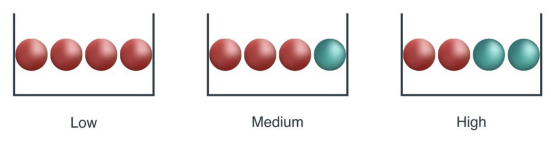
\includegraphics[width=\linewidth]{"Temas/Tema 1/screenshot001.png"}
		\end{minipage}\qquad
		\begin{minipage}{0.35\textwidth}
		Podemos expresar dicha señal de la forma $x(-t+1)$, donde vemos rápidamente que se trata de una inversión y un desplazamiento de un segundo hacia la derecha. Por tanto, tal como se muestra gráficamente en la figura, la señal $x(1-t)$ será cero para $t>-2$.
		\end{minipage}
		\item $\db{x(1-t)+x(2-t)}$
		
		\item $\db{x(1-t)x(2-t)}$
		
		\begin{minipage}{0.55\textwidth}
				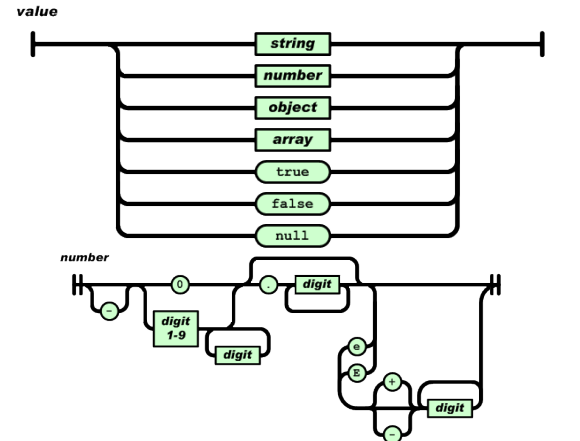
\includegraphics[width=\linewidth]{"Temas/Tema 1/screenshot002.png"}
				\end{minipage}\qquad\begin{minipage}{0.35\textwidth}
				Si la señal $x(1-t)$ es cero para $t>-2$, vemos fácilmente que $x(2-t)$ es cero para $t>-1$. Por tanto, al multiplicarlas, seguirá siendo cero para $t>-2$. En la figura puede verse gráficamente
				\end{minipage}
		\item $\db{x(3t)}$
		\item $\db{x\left(\dfrac{t}{3}\right)}$
	\end{enumerate}
	\item\lb{Determine si cada una de las siguientes señales es periódica:}
	\begin{enumerate}[label=\color{red}\alph*)]
		\item $\db{x(t)=2e^{j(t+\frac{pi}{4})}u(t)}$

		$x(t)=\lbb{2e^{j(t+\frac{pi}{4})}}{\text{per}}\cdot\lbb{u(t)}{\text{no per}}\longrightarrow\text{ no periódica}$

		\item $\db{x[n]=u[n]+u[-n]}$

		$x[n]=u[n]+u[-n]\longrightarrow$ no periódica

		\begin{tikzpicture}
			\foreach \x in {0,...,4}{
					\fill[lightblue] (\x,1) circle (2pt);
					\draw[lightblue] (\x,0) -- (\x,1);
				}
			\draw[-latex] (-2,0) -- (5,0);
			\draw[-latex] (0,-1) -- (0,1.5) node[right] {$x[n]$};
			\foreach \x in {-2,-1}{
					\fill[lightblue] (\x,0) circle (2pt);
				}
		\end{tikzpicture}

		\begin{tikzpicture}
			\foreach \x in {-2,...,0}{
					\fill[lightblue] (\x,1) circle (2pt);
					\draw[lightblue] (\x,0) -- (\x,1);
				}
			\draw[-latex] (-2,0) -- (5,0);
			\draw[-latex] (0,-1) -- (0,1.5) node[right] {$x[-n]$};
			\foreach \x in {1,...,4}{
					\fill[lightblue] (\x,0) circle (2pt);
				}
		\end{tikzpicture}

		\begin{tikzpicture}
			\foreach \x in {-2,...,2}{
					\fill[lightblue] (\x,1) circle (2pt);
					\draw[lightblue] (\x,0) -- (\x,1);
				}
			\draw[-latex] (-2,0) -- (5,0);
			\draw[-latex] (0,-1) -- (0,1.5) node[right] {x[n]+x[-n]};

		\end{tikzpicture}
		\item $\db{x[n]=\sum_{k=-\infty}^{\infty}\left(\delta[n-4k]-\delta[n-1-4k]\right)}$
		
		\begin{tikzpicture}
			\foreach \x in {-4,0,4}{
					\fill[lightblue] (\x,1) circle (2pt);
					\draw[lightblue] (\x,0) -- (\x,1);
				}
			\draw[-latex] (-5.5,0) -- (6.5,0) node[right] {n};
			\draw[-latex] (0,-1) -- (0,1.5);
			\foreach \x in {-5,-3,-2,-1,2,3,5,6}{
					\fill[lightblue] (\x,0) circle (2pt);
				}
			\foreach \x in {-3,1,5}{
					\fill[lightblue] (\x,-1) circle (2pt);
					\draw[lightblue] (\x,0) -- (\x,-1);
				}
		\end{tikzpicture}
	\end{enumerate}
	\item \lb{Para cada una de las señales siguientes determine los valores de la variable independiente en los que se garantice que la parte par de la señal es cero.}
	\begin{enumerate}[label=\color{red}\alph*)]
		\item $\db{x[n]=u[n]-u[n-4]}$
		\item $\db{x(t)=\sin\left(\dfrac{t}{2}\right)}$
		\item $\db{x[n]=\left(\dfrac{1}{2}\right)^nu[n-3]}$
		\item $\db{x(t)=e^{-5t}u(t+2)}$
	\end{enumerate}
	\item \lb{Exprese la parte real de cada una de las siguientes señales de la forma $Ae^{-at}\cos(\omega t+\varphi)$, donde $A,a,\omega$ y $\varphi$ son números reales con $A\ge0$ y $-\pi\le\varphi\le\pi$.}
	\begin{enumerate}[label=\color{red}\alph*)]
		\item $\db{x(t)=-2}$
		\item $\db{x(t)=\sqrt{2}e^{j\frac{\pi}{4}}\cos(3t+2\pi)}$
		\item $\db{x(t)=e^{-t}\sin(3t+\pi)}$
		\item $\db{x(t)=je^{(-2+j100)t}}$
	\end{enumerate}
	\item \lb{Determine si cada una de las siguientes señales es periódica. En caso afirmativo especifiquen su periodo fundamental.}
	\begin{enumerate}[label=\color{red}\alph*)]
		\item $\db{x(t)=je^{j10t}}$

		$x(t)=\lbb{j}{e^{j\frac{\pi}{2}}}e^{j10t}=e^{j\left(10t+\frac{\pi}{2}\right)}\longrightarrow$ periódica

		$\omega_0=10\longrightarrow T=\dfrac{2\pi}{\omega_0}=\dfrac{\pi}{5}$

		\item $\db{x(t)=e^{(-1+j)t}}$

		$x(t)=e^{(-1+j)t}=e^{-t}\cdot e^{jt}\longrightarrow$ no periódica

		\item $\db{x[n]=e^{j7\pi n}}$

		$x[n]=e^{j7\pi n}\longrightarrow$ periódica

		$\omega_0=7\pi\longrightarrow N=\dfrac{2\pi}{\omega_0}K=\dfrac{2\cancel{\pi}}{7\cancel{\pi}}K=\left\{K=7\right\}=2$
		\item $\db{x[n]=3e^{j\frac{3\pi}{5}\left(n+\frac{1}{2}\right)}}$
 
		$x[n]=3e^{j\frac{3\pi}{5}\left(n+\frac{1}{2}\right)}=3e^{j\frac{3\pi}{10}}\cdot e^{j\frac{3\pi}{5}n}$

		$\omega_0=\dfrac{3\pi}{5}\longrightarrow N=\dfrac{2\pi}{\omega_0}K=\dfrac{10\cancel{\pi}}{3\cancel{\pi}}K=\left\{k=3\right\}=10$

		\item $\db{x[n]=3e^{j\frac{3}{5}\left(n+\frac{1}{2}\right)}}$

		$x[n]=3e^{j\frac{3}{5}\left(n+\frac{1}{2}\right)}\longrightarrow$ no periódica
	\end{enumerate}
	\item \lb{Determine el periodo fundamental de la señal $x(t)=2\cos(10t+1)-\sin(4t-1)$.}
	
	$x(t)=2\cos(10t+1)-\sin(4t-1)$
	
		$\begin{array}{l}
				T=k_1\cdot T_1=k_2\cdot T_2  \\
				\begin{rcases}
					x_1=10\longrightarrow T_1=\dfrac{2\pi}{10}=\dfrac{\pi}{5} \\
					w_2=4\longrightarrow T_2=\dfrac{2\pi}{4}=\dfrac{\pi}{2}
				\end{rcases}k_1\dfrac{\cancel{\pi}}{5}=k_2\dfrac{\cancel{\pi}}{2} \\
				2k_1=5k_2\begin{cases}
					k_1=5 \\
					k_2=2
				\end{cases}\longrightarrow\bboxed{T=5\cdot\dfrac{\pi}{5}=\pi}
			\end{array}$
	\item \lb{Determine el periodo fundamental de la señal $x[n]=1+e^{j\frac{4\pi n}{7}}-e^{j\frac{2\pi n}{5}}$.}
	
	\item \lb{Considere la señal en  tiempo discreto $x[n]=1-\sum_{k=3}^{\infty}\delta[n-1-k]$. Determine los valores de los números enteros $M$ y $n_0$ que permite que $x[n]$ pueda expresarse como $x[n]=u[Mn+n_0]$.}
	\item \lb{Considere la señal en tiempo continuo $x(t)=\delta(t+2)-\delta(t-2)$. Calcule la energía de la señal $y(t)=\int_{-\infty}^{t}x(\tau)\mathrm{d}\tau$.}
	\item \lb{La figura 1 muestra la señal continua $x(t)$. Represente cada una de las siguientes señales}

	\begin{figure}[h]
		\centering
		\begin{tikzpicture}
			\draw (-2.5,0) -- (2.5,0) node[below right] {$t$};
			\draw (0,-1.5) -- (0,2.5);
			\draw[draw=lightblue, line width=1.2] (-2,0) node[below left] {-2} -- (-2,-1) -- (-1,0) node[below] {-1} -- (-1,1) -- (0,1) node[right] {1} -- (0,2) node[left] {2} -- (1,2) -- (1,1) -- (2,0) node[below] {2};
			\node[below right] at (0,0) {0};
			\node[right] at (0,-1) {-1};
			\node[below] at (1,0) {1};
		\end{tikzpicture}
		\caption*{Figura 1}
	\end{figure}

	\pagebreak

	\begin{enumerate}[label=\color{red}\alph*)]
			\item \db{$x(t-1)$}
			
			Se trata de un desplazamiento a la derecha de 1 segundo. Es decir, la nueva señal está \textbf{retrasada} un tiempo $t=1$ segundo con respecto a la original, tal como se muestra en la figura.
			
			\begin{center}
			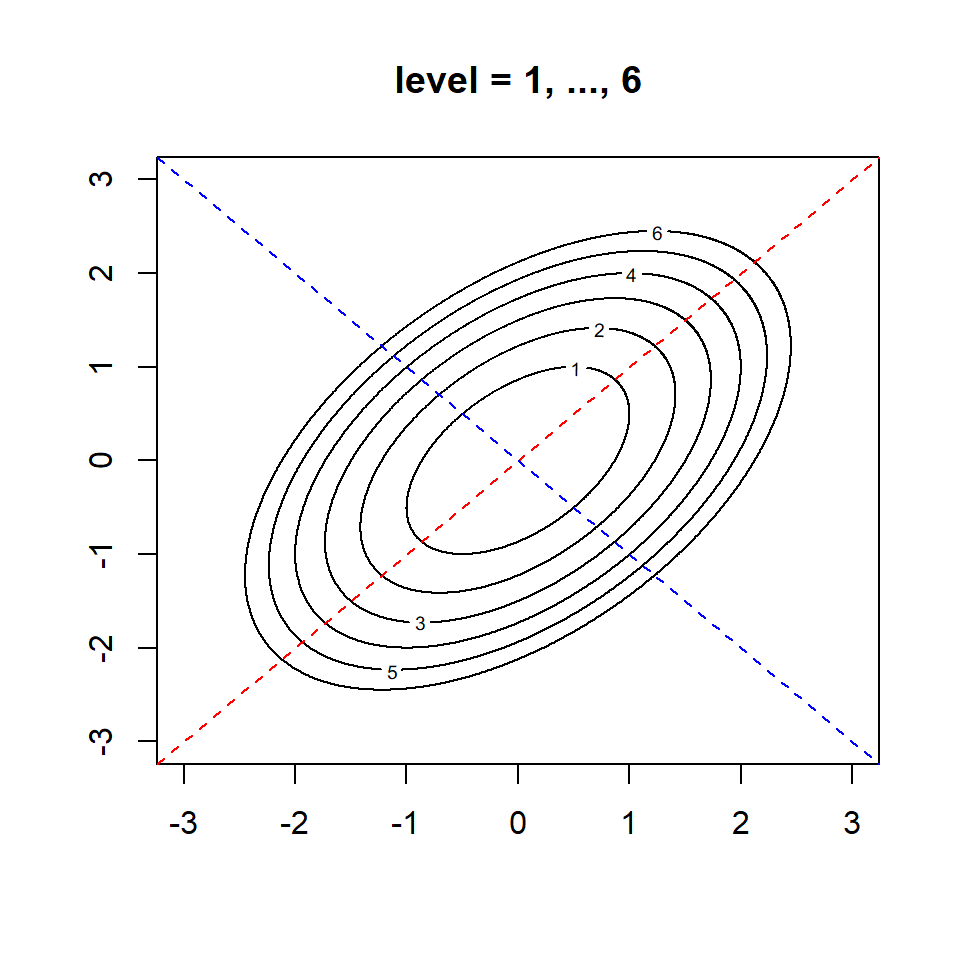
\includegraphics{"Temas/Tema 1/screenshot003.png"}
			\end{center}
			
			\item $\db{x(2-t)}$
			
			Se trata de aplicar la inversión para obtener $x(-t)$ y a continuación aplicar un desplazamiento a la derecha de $t_0=2$ segundos.
			
			\begin{center}
			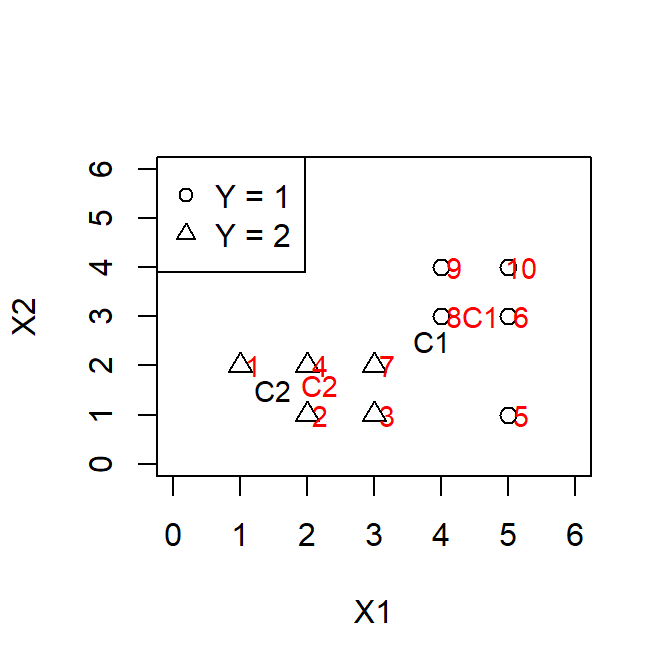
\includegraphics[width=0.7\textwidth]{"Temas/Tema 1/screenshot004.png"}
			\end{center}
			
			\begin{center}
			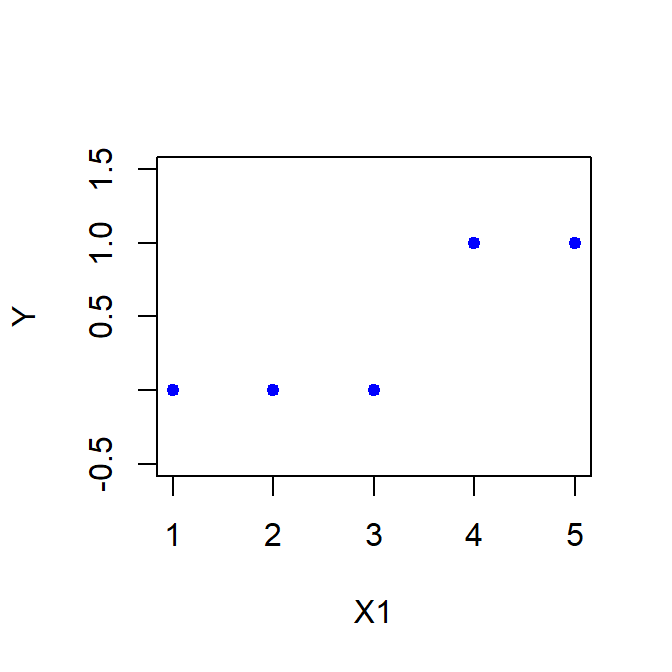
\includegraphics[width=0.7\textwidth]{"Temas/Tema 1/screenshot005.png"}
			\end{center}
			
			\item $\db{x(2t+1)}$
			
			Se trata de aplicar una compresión a la señal $x(t)$ por un factor $a=2$ y a continuación un desplazamiento a la izquierda de $t_0=1$.
			
			Inicialmente se ha aplicado la compresión y a la señal resultante se le ha aplicado el Desplazamiento de $\frac{t_0}{a}=0.5$ segundos
			\begin{center}
				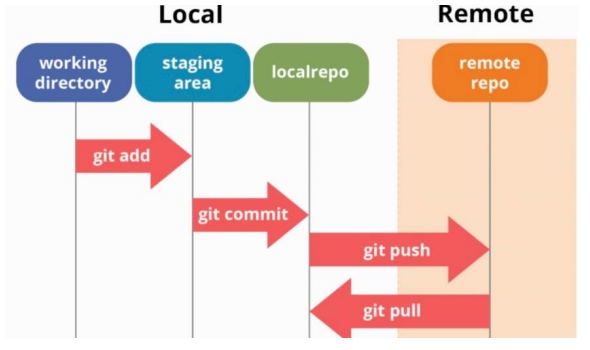
\includegraphics[width=0.7\textwidth]{"Temas/Tema 1/screenshot006.png"}
			\end{center}
			\item $\db{x\left(4-\dfrac{t}{2}\right)}$
			
			Se trata de aplicar una inversión, una expansión a la señal $x(t)$ por un factor $a=\dfrac{1}{2}$ y a continuación un desplazamiento a la derecha de $t_0=4$.
			
			La figura muestra la opción de aplicar, inversión, expansión y luego a la señal resultante la desplazamos una cantidad $\dfrac{t_0}{a}=\dfrac{4}{0.5}=8$ segundos a la derecha.
			
			\begin{center}
			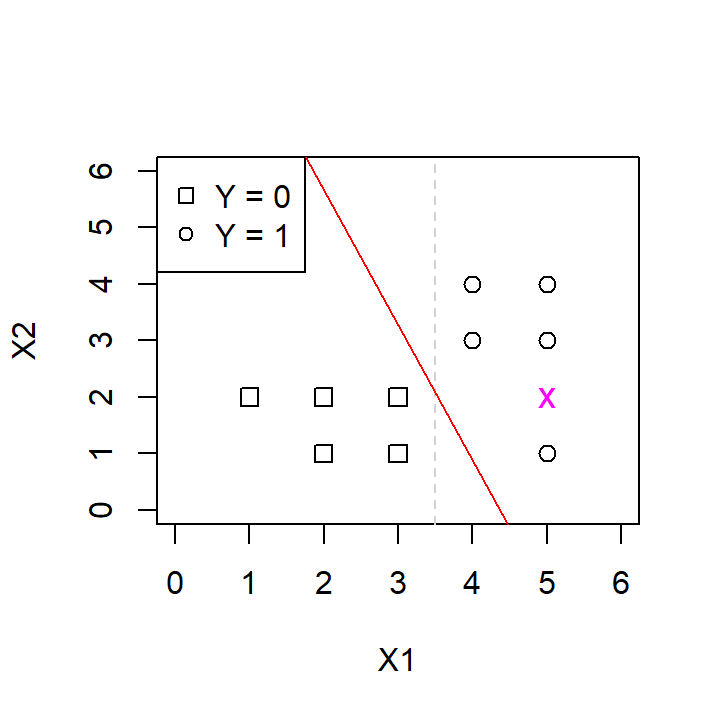
\includegraphics[width=0.6\textwidth]{"Temas/Tema 1/screenshot007.png"}
			\end{center}
			
			\item $\db{[x(t)+x(-t)]u(t)}$
			
			Se trata de sumar la señal $x(t)$ con su invertida y a la resultante se la multiplica por la señal escalón. Esto implica que para $t<0$ será nula.
			
			\begin{center}
			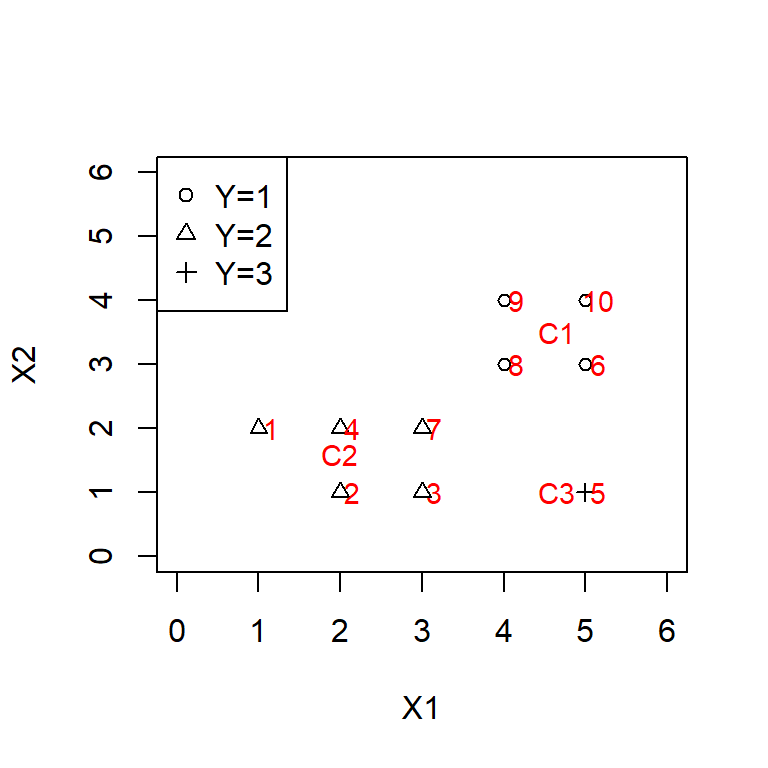
\includegraphics[width=0.7\linewidth]{"Temas/Tema 1/screenshot008.png"}
			\end{center}
			
			\item $\db{x(t)\left[\delta\left(t+\dfrac{3}{2}\right)-\delta\left(t-\dfrac{3}{2}\right)\right]}$
			
			\begin{minipage}{0.55\linewidth}
			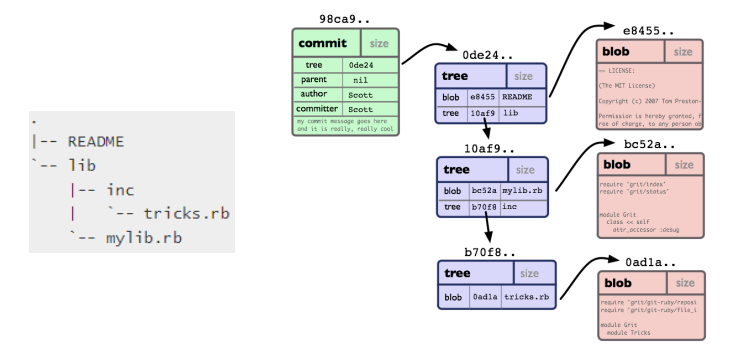
\includegraphics[width=\linewidth]{"Temas/Tema 1/screenshot009.png"}
			\end{minipage}\qquad\begin{minipage}{0.35\textwidth}
			Se trata de la suma de la señal original $x(t)$ multiplicando por dos deltas centradas en $t=-1.5$ segundos y $t=1.5$ segundos, tal como se muestra en la figura. La salida son dos deltas ponderadas por el valor de $x(t)$ en $t_0=-1.5$ y $t_1=1.5$
			\end{minipage}
		\end{enumerate}
		\item \lb{La figura 2 muestra la señal discreta $x[n]$. Representa cada una de las siguientes señales:}
		\begin{figure}[h]
			\centering
			\begin{tikzpicture}
				\draw (-6,0) -- (6,0);
				\foreach \x in {-5.5, 5.5}{\node[above] at (\x,0) {$\cdots$};}
				\foreach \x in {-5, 4, 5}{
				\fill[lightblue] (\x,0) circle (2pt) node[below] {$\x$};
				}
				\foreach \x in {-2,3}{\draw[lightblue, -*] (\x, 0) node[below] {$\x$} -- (\x,0.5) node[above] {$\frac{1}{2}$};}
				\foreach \x in {-1,0,...,2}{\draw[lightblue, -*] (\x,0) node[below] {$\x$} -- (\x,1);}
				\draw[lightblue, -*] (-4,0) node[below left] {$-4$} -- (-4,-1) node[below] {$-1$};
				\draw[lightblue, -*] (-3,0) node[below left] {$-3$} -- (-3,-0.5) node[below] {$-\frac{1}{2}$};
			\end{tikzpicture}
			\caption*{Figura 2}
		\end{figure}
		\begin{enumerate}[label=\color{red}\alph*)]
			\item $\db{x[n-4]}$
			\item $\db{x[3-n]}$
			\item $\db{x[3n]}$
			
			\begin{minipage}{0.55\textwidth}
				\begin{center}
				\includegraphics[width=\linewidth]{"Temas/Tema 1/screenshot010"}
				
				\includegraphics[width=\linewidth]{"Temas/Tema 1/screenshot011"}
			\end{center}
			\end{minipage}\qquad\begin{minipage}{0.35\textwidth}
			Se trata de una compresión en el tiempo por un factor de $a=3$. La duración de la señal se reduce un tercio.\\
			Se puede considerar que ahora el periodo de muestreo se baja a un tercio.
			
			\end{minipage}
			
			\item $\db{x[3n+1]}$
			
			\begin{minipage}{0.55\textwidth}
				\begin{center}
				\includegraphics[width=\linewidth]{"Temas/Tema 1/screenshot010"}
				
				\includegraphics[width=\linewidth]{"Temas/Tema 1/screenshot012"}
			\end{center}
			\end{minipage}\qquad\begin{minipage}{0.35\textwidth}
			Se trata de una compresión en el tiempo por un factor de $a=3$ y un desplazamiento.\\
			Primero se aplica el desplazamiento y después la compresión.
			\end{minipage}
			
			\item $\db{x[n]u[3-n]}$
			\item $\db{x[n-2]\delta[n-2]}$
			\item $\db{\dfrac{1}{2}x[n]+\dfrac{1}{2}(-1)^nx[n]}$
			\item $\db{x[(n-1)^2]}$
		\end{enumerate}
\end{enumerate}